\documentclass[letterpaper,11pt]{article}

\usepackage{listings}
\usepackage{color}

\definecolor{dkgreen}{rgb}{0,0.6,0}
\definecolor{gray}{rgb}{0.5,0.5,0.5}
\definecolor{mauve}{rgb}{0.58,0,0.82}

\lstset{frame=tb,
  language=Python,
  aboveskip=3mm,
  belowskip=3mm,
  showstringspaces=false,
  columns=flexible,
  basicstyle={\small\ttfamily},
  numbers=none,
  numberstyle=\tiny\color{gray},
  keywordstyle=\color{blue},
  commentstyle=\color{dkgreen},
  stringstyle=\color{mauve},
  breaklines=true,
  breakatwhitespace=true,
  tabsize=3
}

\usepackage{setspace}
\usepackage{graphicx}
\usepackage{bm}    %for textbf
\usepackage{amsmath}
\usepackage{amsfonts}   %for mathbb
\allowdisplaybreaks[4]  %from {amsmath}
\newcommand{\independent}{\rotatebox[origin=c]{90}{$\models$}}  %from {graphicx}
\usepackage{geometry}
\geometry{letterpaper, scale=0.8}  %from {geometry}
\author{Yuan Yin}
\title{EECS 545 Homework 3}
\begin{document}\large
\maketitle
\begin{spacing}{1.2}  %from {setspace}
\section*{Problem 2}
\subsection*{(b) \& (c)}
The code and result is as follows:
\begin{lstlisting}
import numpy as np
import matplotlib.pyplot as plt
import pylab as pl

n = 200
np.random.seed(0) # Seed the random number generator
x = np.random.rand(n,1)
z = np.zeros([n,1])
k = n * 0.4
rp = np.random.permutation(n)
outlier_subset = rp[1:int(k)]
z[outlier_subset] = 1 # outliers
y = (1 - z) * (10 * x + 5 + np.random.randn(n,1)) + z * (20 - 20 * x + 10 * np.random.randn(n,1))

# Plot data and true line
plt.scatter(x, y, label = 'data')

t = pl.frange(0,1,0.01)
plt.plot(t, 10*t+5, 'k-', label = 'true line')

# Add your code for ordinary least squares below
x_ols = np.mat(x); y_ols = np.mat(y) # They are all 200*1 matrix
y_mdf = y_ols - np.mean(y_ols); x_mdf = x_ols - np.mean(x_ols)
A = 2 * (x_mdf.T * x_mdf); r = -2 * x_mdf.T * y_mdf; c = y_mdf.T * y_mdf
w_ols = -(A.I * r)[0,0]; b_ols = np.mean(y_ols) - w_ols * np.mean(x_ols)
print("Parameters of OLS are: w: ",w_ols, "b: ", b_ols)

plt.plot(t, w_ols*t+b_ols, 'g--', label = 'least squares')

#######################################################
# helper function to solve weighted least squares
    # add your code here
def wls(x,y,c):
    add = 1
    x_add = np.insert(x, 0, values=add, axis=1)
    theta = (x_add.T * c * x_add).I * x_add.T * c * y
    b = theta[0]; w = theta[1]
    return w, b

# Add your code for robust regression MM algorithm below
x_rob = np.mat(x); y_rob = np.mat(y)
w_rob = 0; b_rob = 0
error = 1
while error > 0.01:
    c = np.eye(len(x_rob))
    for i in range(len(x_rob)):
        r_t_i = y_rob[i] - w_rob * x_rob[i] - b_rob
        c[i,i] = 1/(2*np.sqrt(1+r_t_i**2))
    w_new, b_new = wls(x_rob, y_rob, c)
    error = np.sqrt((w_new - w_rob)**2 + (b_new - b_rob)**2)
    w_rob, b_rob = w_new[0,0], b_new[0,0]

print("Parameters of ROB are: w: ",w_rob, "b: ", b_rob)
plt.plot(t, w_rob*t+b_rob, 'r:', label = 'robust')
legend = plt.legend(loc='upper right', shadow=True)
plt.show()
\end{lstlisting}
The result is:
\begin{lstlisting}
Parameters of OLS are: w: -1.4749427077811519 b: 10.519708850514508
Parameters of robust regression are: w: 7.302235544182917 b: 6.186315755157274
\end{lstlisting}
The plot which shows the data, the true line, the OLS estimate and the robust estimate is as bellow:

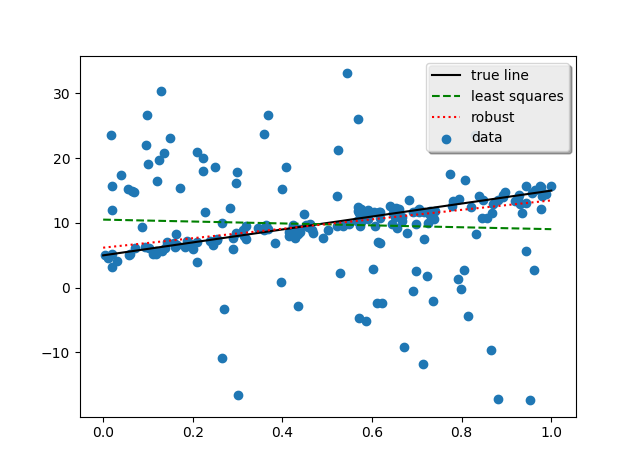
\includegraphics[width=4.95in,height=4.05in]{Robust_Regression.png}

\section*{Problem 4}
\subsection*{(b)}
The code and the result is as follows:
\begin{lstlisting}
import numpy as np
import scipy.io as sio
import matplotlib.pyplot as plt
import pylab as pl

np.random.seed(0) # Seed the random number generator
# Load the data
nuclear = sio.loadmat('nuclear.mat')
x = nuclear['x']
y = nuclear['y'] # 1 represents neutrons and -1 represents gamma rays
d,n = x.shape

# Plot data
gamma_rays = []; neutrons = []
for i in range(n):
    if y[0,i] == 1:
        neutrons.append(i)
    else:
        gamma_rays.append(i)
plt.figure()
plt.scatter(x[0,gamma_rays], x[1,gamma_rays], s = 1, label = 'data of gamma rays')
plt.scatter(x[0,neutrons], x[1,neutrons], s = 1, c = 'r', label = 'data of neutrons')

# Initialization and plot learned line
x = np.mat(x); y = np.mat(y)
add = 1; J = []
x_tilda = np.insert(x, 0, values=add, axis=0)
lamda = 0.001; omega = np.zeros(d); b = 0
Iteration = 35
for j in range(Iteration):
    u = 0; alpha = 100/(j+1); Loss = 0
    for i in range(n):
        h = 1 - y[0,i] * (np.dot(omega, x[:,i]) + b)
        if h[0,0] > 0:
            scale = 1
        elif h[0,0] < 0:
            scale = 0
        else:
            scale = np.random.rand()
        u += 1/n * (-y[0,i] * x_tilda[:,i]) * scale + lamda / n * np.mat([0, omega[0], omega[1]]).T
        Loss += max(0, h[0,0])
    J.append(Loss/n + lamda/2 * np.dot(omega, omega))
    b -= alpha * u[0]; omega[0] -= alpha * u[1]; omega[1] -= alpha * u[2]

print(b[0,0], omega[0], omega[1])
t = pl.frange(0,8,0.01)
n = pl.frange(1,Iteration)
plt.plot(t, -omega[0]/omega[1] * t - b[0,0]/omega[1], label = 'learned line')
legend = plt.legend(loc='upper right', shadow=True)
# Plot the objective function
plt.figure()
plt.plot(n, J, label = 'Objective Function')
plt.show()
\end{lstlisting}
The result is:
\begin{lstlisting}
Parameters of estimated hyperplane are:
b = -1.1543275085302598 w_1 = -3.8809615376043824 w_2 = 18.631005972691405
the minimum achieved value of the objective function is: 0.3590574177462417
\end{lstlisting}
The plots showing the data and the learned line, and showing J as a function of iteration number is as bellow:

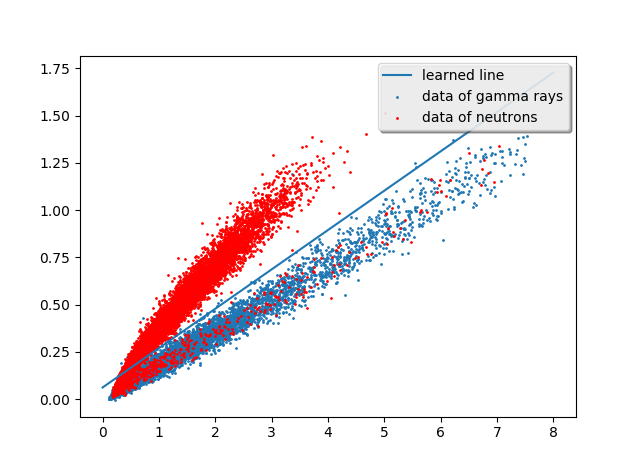
\includegraphics[width=4.95in,height=4.05in]{sg_opt_smh.png}

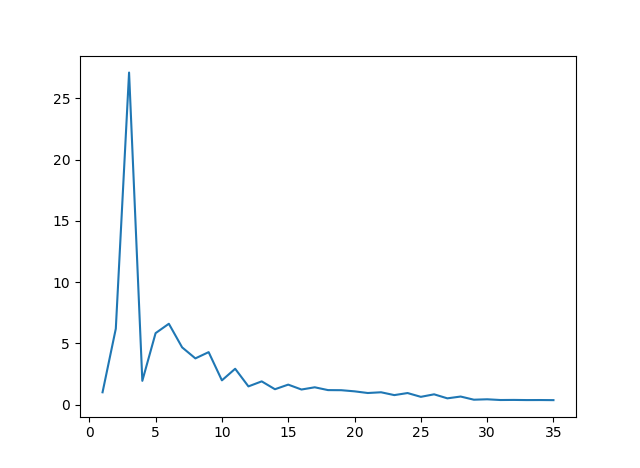
\includegraphics[width=4.95in,height=4.05in]{sg_opt_smh_J.png}

\subsection*{(c)}
the code and the result is as follows:
\begin{lstlisting}
import numpy as np
import scipy.io as sio
import matplotlib.pyplot as plt
import pylab as pl

np.random.seed(0) # Seed the random number generator
# Load the data
nuclear = sio.loadmat('nuclear.mat')
x = nuclear['x']
y = nuclear['y'] # 1 represents neutrons and -1 represents gamma rays
d,n = x.shape

# Plot data
gamma_rays = []; neutrons = []
for i in range(n):
    if y[0,i] == 1:
        neutrons.append(i)
    else:
        gamma_rays.append(i)
plt.figure()
plt.scatter(x[0,gamma_rays], x[1,gamma_rays], s = 1, label = 'data of gamma rays')
plt.scatter(x[0,neutrons], x[1,neutrons], s = 1, c = 'r', label = 'data of neutrons')

# Initialization and plot learned line with stochastic sub-gradient method
x = np.mat(x); y = np.mat(y)
add = 1; J = []
x_tilda = np.insert(x, 0, values=add, axis=0)
lamda = 0.001; omega = np.zeros(d); b = 0
Iteration = 35
for j in range(Iteration):
    ui = 0; alpha = 100/(j+1); N = np.random.permutation(n); Loss = 0
    for i in N:
        h = 1 - y[0,i] * (np.dot(omega, x[:,i]) + b)
        if h[0,0] > 0:
            scale = 1
        elif h[0,0] < 0:
            scale = 0
        else:
            scale = np.random.rand()
        ui = 1/n * (-y[0,i] * x_tilda[:,i]) * scale + lamda / n * np.mat([0, omega[0], omega[1]]).T
        b -= alpha * ui[0]; omega[0] -= alpha * ui[1]; omega[1] -= alpha * ui[2]
        t = (omega * x + b)
        Loss = np.array(1 - np.multiply(y, t))
        Loss *= (Loss > 0)
        # Loss += max(0, h[0, 0])
        J.append(np.sum(Loss)/n + lamda/2 * np.dot(omega, omega))

print("Parameters of estimated hyperplane are: b = ", b[0,0], "w_1 = ", omega[0], "w_2 = ", omega[1])
print("the minimum achieved value of the objective function is: ", min(J))
t = pl.frange(0,8,0.01)
n = pl.frange(1,Iteration*n)
plt.plot(t, -omega[0]/omega[1] * t - b[0,0]/omega[1], label = 'learned line')
legend = plt.legend(loc='upper right', shadow=True)

# Plot the objective function
plt.figure()
plt.plot(n, J, label = 'Objective Function')
plt.show()
\end{lstlisting}
The result is:
\begin{lstlisting}
Parameters of estimated hyperplane are: b =  -0.9463755603126593 w_1 =  -2.200214343271486 w_2 =  11.238670609411892
the minimum achieved value of the objective function is:  0.29596596817675697
\end{lstlisting}

The plots showing the data and the learned line, and showing J as a function of iteration number is as bellow:

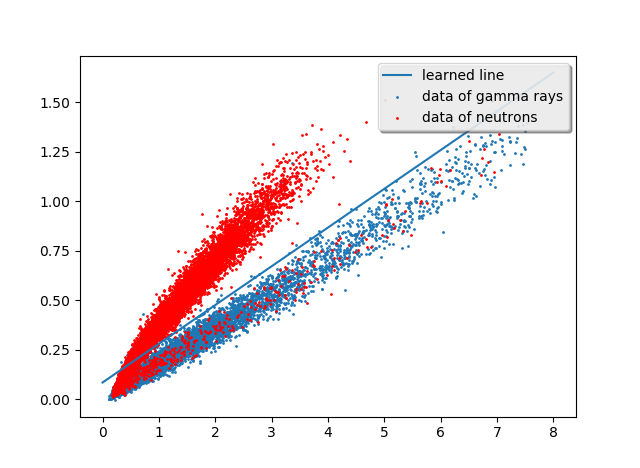
\includegraphics[width=4.95in,height=4.05in]{sto_sg_opt_smh.png}

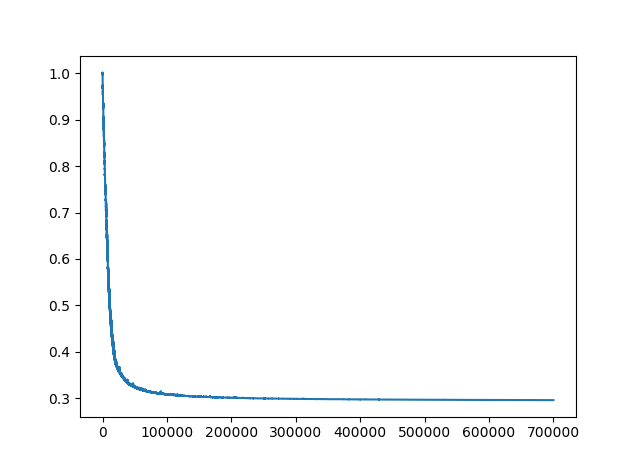
\includegraphics[width=4.95in,height=4.05in]{sto_sg_opt_smh_J.png}

\end{spacing}
\end{document}